%!TEX root = ../report.tex

\section{Network Layer}
The network layer serves the following functions:
\begin{itemize}
  \item IP protocol for addressing, datagram format and packet handling conventions
  \item Routing protocols for path selection
  \item ICMP protocol for error reporting and router signaling
\end{itemize}

\subsection{Internet Protocol}
\begin{figure}[H]
  \centering
  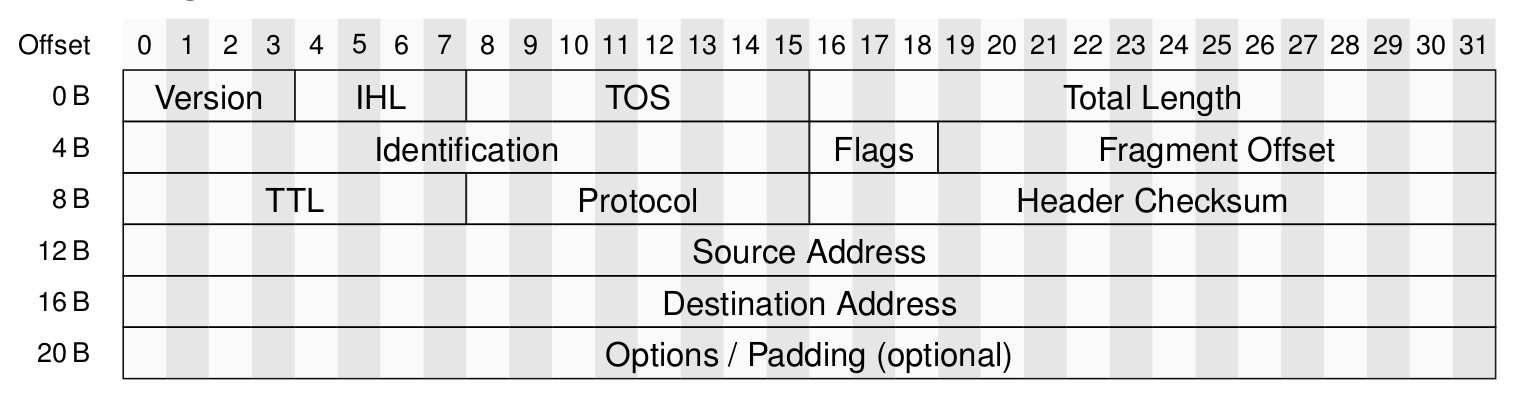
\includegraphics[width=.8\textwidth]{figures/ipv4_datagram.png}
  \caption{IPv4 Datagram}\label{fig:ipv4_datagram}
\end{figure}

\subsubsection*{IPv4 Addressing}
IPv4 addresses are 32-bit identifiers for every host and router interfaces where interfaces represent the connection between host/router and physical link.

Subnets are device interfaces with the same subnet part of the IP address which can physically reach each other without intervening router.

Splitting the IP address into network and host part is done in the following way (for the address 192.168.128.1/17):
\begin{figure}[H]
  \centering
  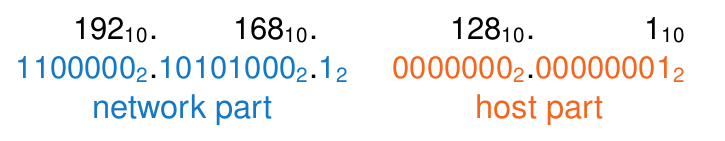
\includegraphics[width=.6\textwidth]{figures/ip_split.png}
\end{figure}

From 1982 to 1993, IP addresses were classfully divided as shown in Figure~\ref{fig:classful_ips}.
\begin{figure}[h]
  \centering
  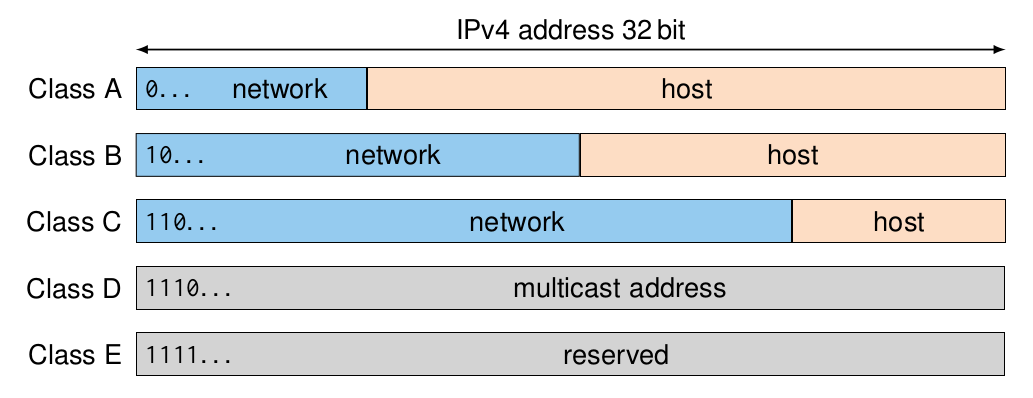
\includegraphics[width=.8\textwidth]{figures/classful_ip.png}
  \caption{Classful IPs}\label{fig:classful_ips}
\end{figure}
In 1993, Classless Inter-Domain Routing (CIDR) was introduced which allowed arbitrary subnet length.
To route packets, prefix matching is used which checks which entry in the routing table fits best for the incoming packet's network prefix.

\subsection{ICMP}
The Internet Control Message Protocol (ICMP) are located above IP but can be considered as part of the IP layer.
It is used for communicating error messages and other attention requiring conditions for IP and TCP or UDP\@.
Two classes of ICMP messages are possible:
\begin{enumerate}
  \item Query messages: only kind that generates other ICMP messages
  \item Error messages: contain IP header and first 8 bytes (today as much as possible up to 572 bytes) of datagram that caused the ICMP message which allows the receiver to put it into context
\end{enumerate}
The structure of an ICMP message is shown in Figure~\ref{fig:icmp_message}.
\begin{figure}[H]
  \centering
  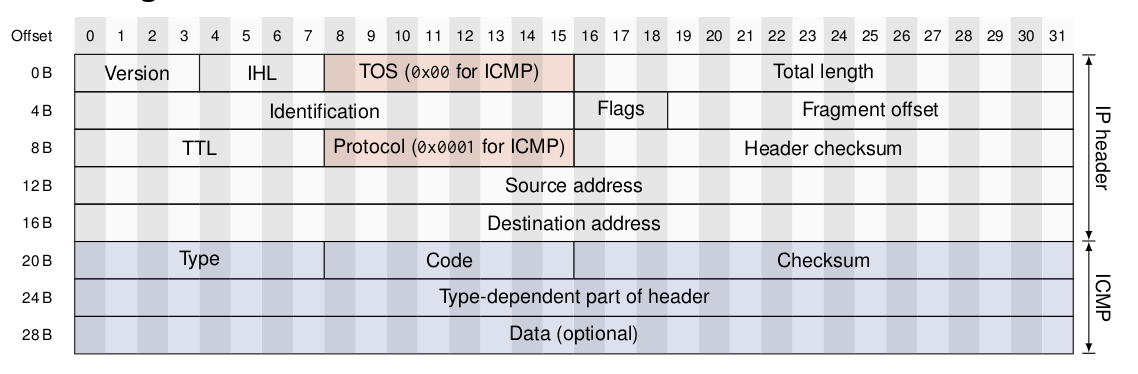
\includegraphics[width=.8\textwidth]{figures/icmp_message.png}
  \caption{ICMP Message}\label{fig:icmp_message}
\end{figure}

